\chapter{Current Implementation}
\label{chapter:myImplementation}

%1. for non smooth solutions and more complex problems theory is still missing. Here like for the standard grid adaptive refinement seems to be necessary to get around solution method. First attempts in this direction are promising\cite{Griebel1992b} \\
%
%2. Consequently, one of the main advantages of the combination technique stems from the properties of sparse grids [1] In comparison to the standard full grid approach the number of grid points can be reduced significantly. Another advantage has to be seen in the simplicity of the combination concept its inherent parallel structure and its framework property allowing the integration of existing solvers for partial differential equations.\cite{Bungartz1994}\\ % write however the idea is in some way different in current implementation
%
%3. we have implicitly assumed that this is the coarse mesh with spacing h that is naturally embedded in the fine mesh, so that the fine mesh solution may be transferred to the coarse mesh with injection.
%
%4. In elliptic problems the smoothness of the solution may be disturbed where the data is non-smooth. The form of the domain or the need for local refinement may make the use of uniform meshes difficult.  The local smoothness of the solution is a basic characteristic of many elliptic problems, so that extrapolation can be used locally, even when the global solution is non-smooth. With this background, several interesting new extrapolation-based approaches have been developed within the past few years, including the sparse grid combination technique and multivariate extrapolation. In this paper we will focus on explicit extrapolation methods that are based on the (linear) combination of solutions on different grids. Implicit extrapolation methods, in contrast, obtain higher order by applying the extrapolation idea on quantities like the truncation error or the numerical approximation of the functional. Such methods are discussed in Rude\cite{Rude1994, Rude92extrapolationand} \\
%
%5. Using bilinear interpolation for each single component function, we can extend the the domain of definition to the union of all participating grids. This is possible, because bilinear interpolation can be shown to be compatible with the error splitting.\cite{Rude1994} \\
%
%6. Obviously, an algorithm is needed which combines the advantages of both methods: low storage requirements, a low number of operations involved, but still simple data structures. In the following, we present an algorithm that fulfills these requirements\cite{Griebel1995} \\
%
%7. Firstly, the block structure of a grid reduces main memory requirements. In an inner iteration step, the problem is solved one block at a time. An outer iteration establishes the overall solution. Secondly, the block structure of a grid is a natural basis for the parallelization of the solver. Each processor solves the problem on one of the blocks, and communication is necessary merely along block interfaces, in order to achieve a smooth solution on the whole domain.\cite{Griebel1995} \\
%
%8. The hierarchical coefficient or hierarchical surplus itself can be used to indicate the smoothness of u at the corresponding grid point and, consequently, the necessity to refine the grid here.\cite{Bungartz1998}\\
 
 \section{General Ideas}
 
 		
		Productivity experts claim that breakthroughs come by thinking "nonlinearly". Tree structures have been an enormous leap in data organization since they allow the implementation of algorithms more rapidly than linear data structures such as lists, vectors and sequences.
		
		In categorizing trees as "nonlinear" with respect to organizational relationship, the main feature that must be highlighted is more sophisticated relationships than elementary "before" and "after" relationships between objects in sequences. A tree follows a \textbf{hierarchical} architecture, with some objects being "above" and some "below" others.
		
		A \textbf{tree} is an abstract data type. In a tree, each element has a \textbf{parent} element. It can have zero or more \textbf{children} elements.
		\\
		\textbf{Formal Tree Definition}
		
		A \textbf{tree T} can be defined as a set of \textbf{nodes} storing elements in a \textbf{parent-child} relationship and has the properties as defined below:
		\begin{itemize}
			\item A nonempty \textbf{T} has a special node known as the \textbf{root} of \textbf{T} which has no parent. 
			\item Every other node \textit{$\nu$} of \textbf{T} has a unique parent node \textit{w} and every node with parent \textit{w} is a \textbf{child} of \textit{w}.
		\end{itemize}

		If a parent has two nodes which are its children, then these children are \textbf{siblings}. If a node \textit{$\nu$} does not have children then it is \textbf{external} while it is \textbf{internal} if it has one or more children. External nodes can also be termed as \textbf{leaves}.
		
		Figure \ref{fig:GeneralTree} shows an example of a tree representing computer files organized in the form of nested directories. 
		
		\begin{figure}[h]
			\centering
			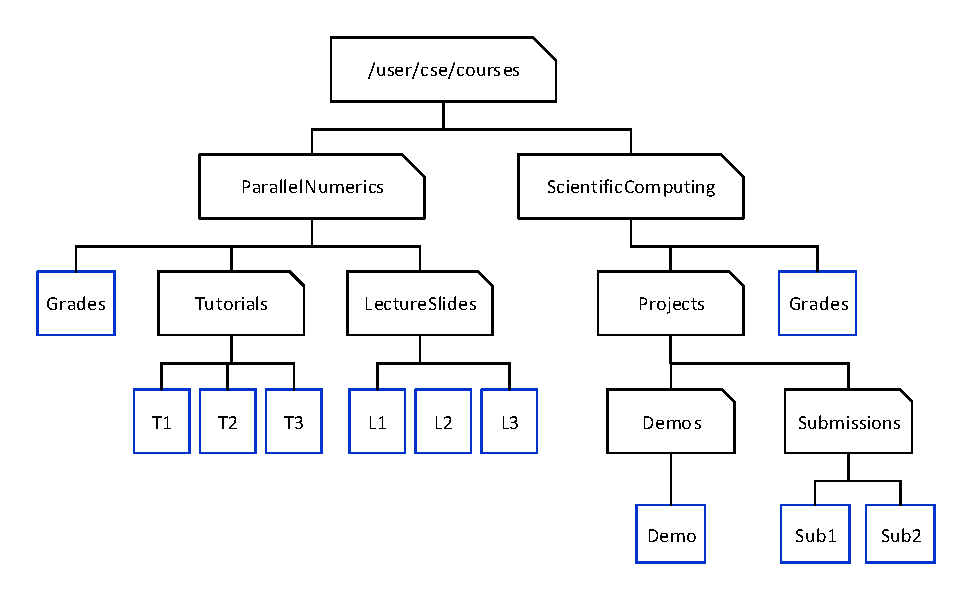
\includegraphics[width=\textwidth]{/GeneralTree.pdf}
			\caption{Tree representing a portion of a file system}
			\label{fig:GeneralTree}
		\end{figure}
		
		\textbf{Ordered Trees}
		
		A tree having a linear ordering for the children of each node is termed as \textbf{ordered}. The children of a node  can be identified as first, second and so on. In ordered trees, linear order relationship between siblings is illustrated by listing them in a sequence.
		
		For implementation "position" and "node" can be used interchangeably for trees. \\
		
		\textbf{A Linked Structure for General}
		
		A \textbf{linked structure} can be used to comprehend a tree \textbf{T}. Each node of \textbf{T} can be depicted as a position object \textit{p} with the below mentioned fields:
		reference to the node's element, link to node's parent and some kind of collection to store links into node's children.  Figure \ref{fig:LinkedStrucGenTree} shows a representation of  a node of a tree and a schematic representation of the data structure associated with a node and its children. \\
		
		% The height of a tree is equal to the maximum depth of its external nodes.
		\begin{figure}[h]
			\centering
		    \begin{subfigure}[b]{0.33\textwidth}
			    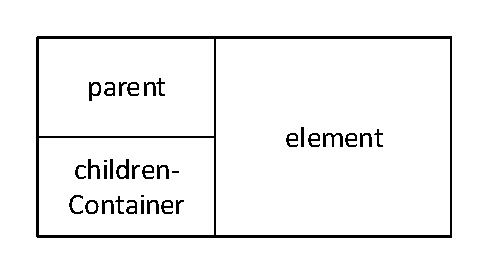
\includegraphics[width =\textwidth]{/LinkedStrucGenTree1.pdf}
			    %\vspace{3em}
				\centering
		        \caption{}
		    \end{subfigure} 
		    \begin{subfigure}[b]{0.66\textwidth}    
			    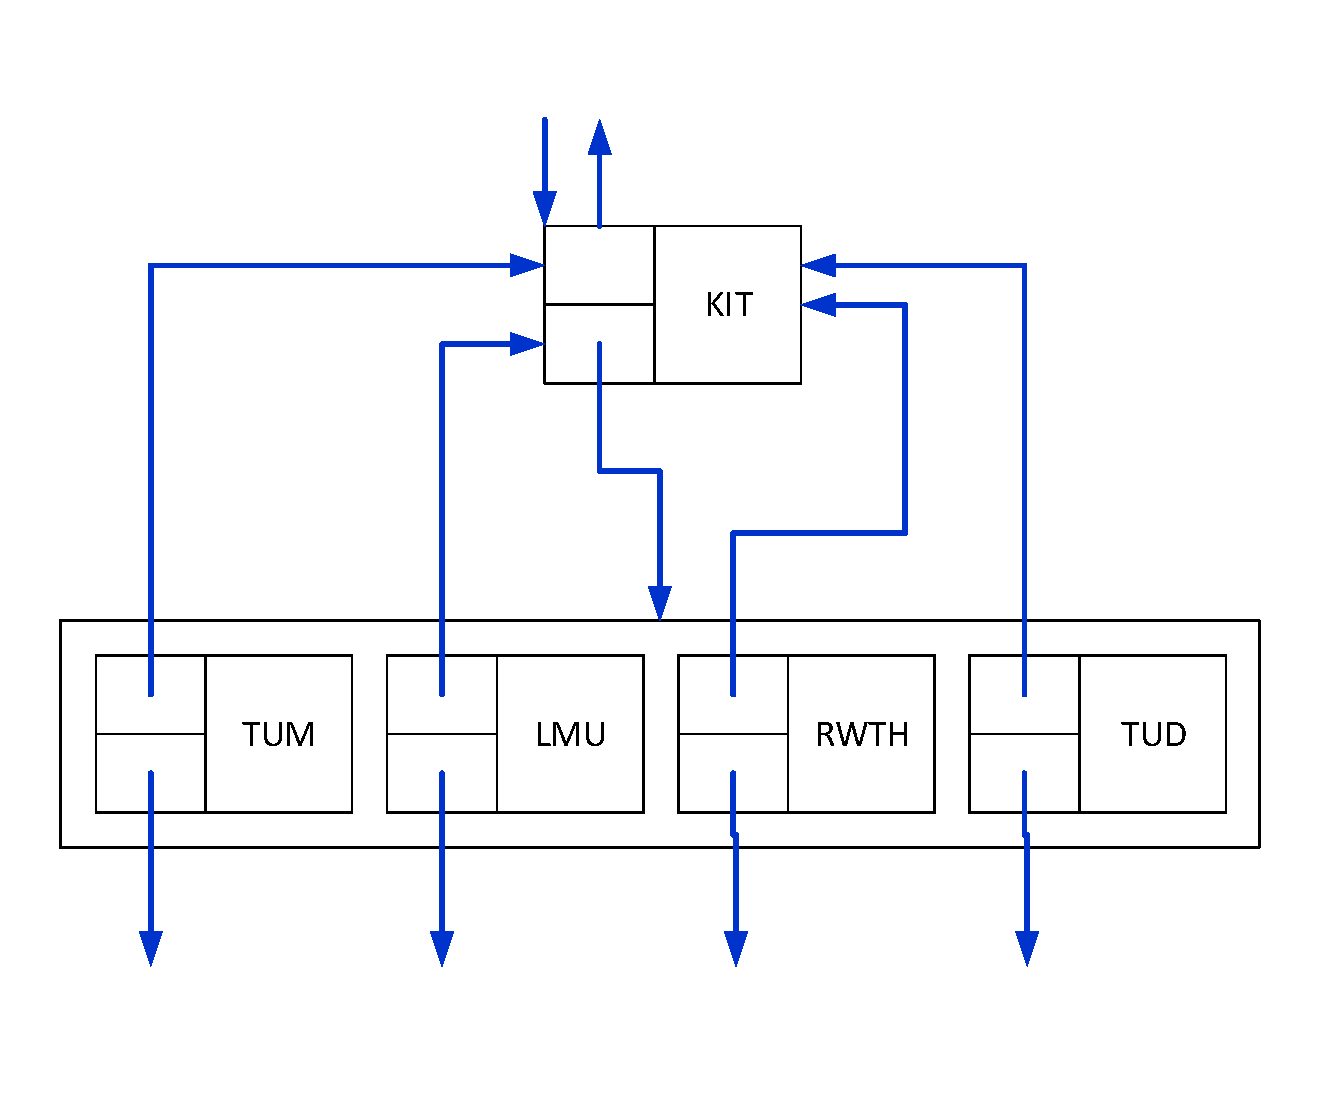
\includegraphics[width =\textwidth]{/LinkedStrucGenTree2.pdf}
				\centering    
			 \caption{}
		    \end{subfigure} 
		    \caption{The linked structure for a general tree: (a) the node structure; (b) the portion of the data structure associated with a node and its children.}
		    \label{fig:LinkedStrucGenTree}
		\end{figure}
		
		
		\textbf{Preorder Traversal}
		
		A traversal of a tree \textbf{T} is a method of acquiring all the nodes of \textbf{T}. Preorder traversal which is a basic traversal scheme for trees has been represented here.\\
		In a preorder traversal of \textbf{T}, the root of \textbf{T} is called initially and further the subtrees rooted at its children are traversed repeatedly. In an ordered tree, the subtrees are traversed according to the order of the children. The definitive action associated with the "visit" of a node depends on the application of this traversal.\\
		
		\textbf{Algorithm}  preorder(T, p):\\
		perform the "visit" action for node p\\
		for each child q of p do\\
		recursively traverse the subtree rooted at q by calling preorder (T,q)\\ 
		
		This algorithm is suitable for creating a linear ordering of the nodes of a tree in which parents always come before their children.\\
		
		The preorder traversal is an effective way to access all the nodes of a tree.\\
		
		Figure \ref{fig:TransversalOrderedTree} shows an example of the preorder traversal of the tree associated with a research paper. The document is sequentially read from beginning to the end.
		
				\begin{figure}[h]
				\centering
					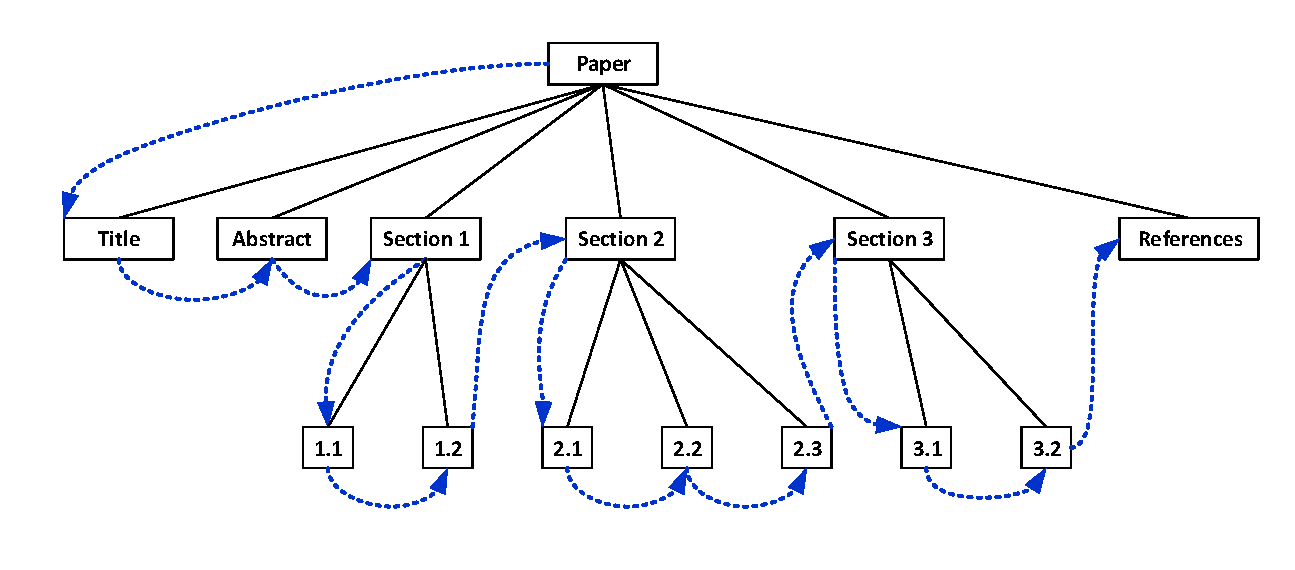
\includegraphics[width=\textwidth]{/TransversalOrderedTree.pdf}
					\caption{Preorder traversal of an ordered tree, where the children of each node are ordered from left to right.}
					\label{fig:TransversalOrderedTree}
				\end{figure}
		
		\textbf{Quad Trees}\\
		
		A \textbf{quad tree} is an ordered tree in which each node has at most four children
		\begin{enumerate}
			\item Every node has at most four children.
			\item Each child node can be labeled as south-west(SW), south-east(SE), north-west(NW) or north-east(NE).
			\item The ordering of a node is implemented as SW$\rightarrow$SE$\rightarrow$NW$\rightarrow$NE. 
		\end{enumerate}
		A quad tree is termed to be \textbf{proper} if each node has either zero or four children.\\
		
		\textbf{A Recursive Quad Tree Definition}\\
		A recursive quad tree can be defined as a quad tree which
		\begin{itemize}
			\item is either empty
			\item consists of a node which is \textbf{root} and four further quad trees which are called as south-west(SW), south-east(SE), north-west(NW) or north-east(NE) subtrees. 
		\end{itemize}
		 
		 Figure \ref{fig:NodeQuadTree} shows a representation of a node in a linked data structure for representing a quad tree.
		 		
		 \begin{figure}[h]
		 	\centering
		 	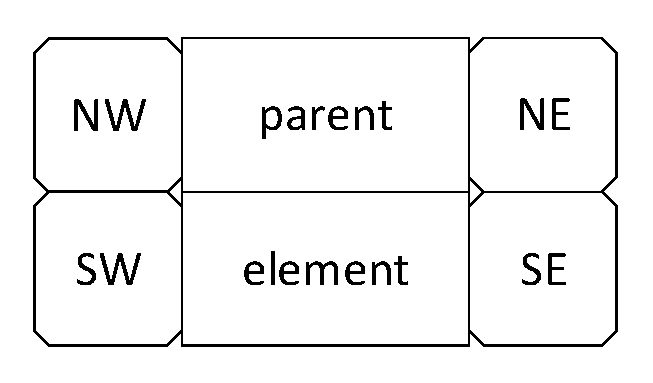
\includegraphics[width=0.33\textwidth]{/NodeQuadTree.pdf}
		 	\caption{A node in a linked data structure for representing a quad tree.}
		 	\label{fig:NodeQuadTree}
		 \end{figure}

 
 \section{Different Schemes}
 


